\chapter{Gas Electron Multiplier Detectors}
\label{chap:II-1-gem}

  In 1968, G. Charpak revolutionized the field of tracking detectors by introducing the Multiwire Proportional Chamber (MWPC). MWPCs were more reliable than the existing single-wire gas counters providing a higher sub-mm resolution and rate capabitilies up to fluxes of several MHz cm$^{-2}$. Developments of manufacturing technics and high-density electronics led to a new generation of detectors fulfilling the needs of high-energy physics experimentation. However, their use in high-luminosity experiments revealed some intrensic weaknesses: the mechanical design of the chamber limits the spacial resolution; long ion drift times affect the efficiency of the detector at high fluxes; solid deposits aglomerate on the wires due to aging and induce sparks in the chamber. \\

  Twenty years later, Micro-Strip Gas Counters (MSGCs) were developped using photolithographic processes to engrave anode and cathode strips on an insulating support. Both the position resolution and the rate capability were increase by several orders of magnitude. Unfortunalty, the detectors were prone to the effect of aging and discharges, irremediably damaging the counters. \\

  The relative success of the MSGCs led to the development of Micro-Pattern Gas Detectors (MPGDs) less suseptible to discharges and offering comparable performances. They make use of micro pattern structures to amplify the signal and reduce the probability of sparks inside the chamber. Two technologies have proven to be operationnal: the micro-mesh gaseous structure (MICROMEGAS) and the Gas Electron Multiplier (GEM) \cite{SAULI1997531}. \\

  Already in use in the COMPASS and TOTEM experiments at CERN, GEM detectors have proven to meet the requirements of high-luminosity environments. In 2009, a dedicated R\&D program was launched to study the feasability of the installation of GEMs in the muon spectrometer of CMS to instrument the positions left vacant by RPCs. In 2016, the so called GE1/1 muon detector upgrade project was approved by CMS to be installed during LS2.

  \section{Motivations for the GE1/1 Muon Detector Upgrade}

    During LS2 in 2018-2019, the CMS GEM collaboration \cite{Colaleo:2021453} will install an additional set of muon detectors in CMS in the 1.6 < |$\eta$| < 2.2 region. The so-called GE1/1 detector will be installed near the ME1/1 CSCs station as shown in Figure \ref{fig:II-1-gem-ge11} which highlights the location of the chamber within the muon spectrometer. The naming convention is identical to the one of the CSCs, namelly GEx/y where x denotates the disk number and y the ring number. \\

    \begin{figure}[h!]
      \centering
      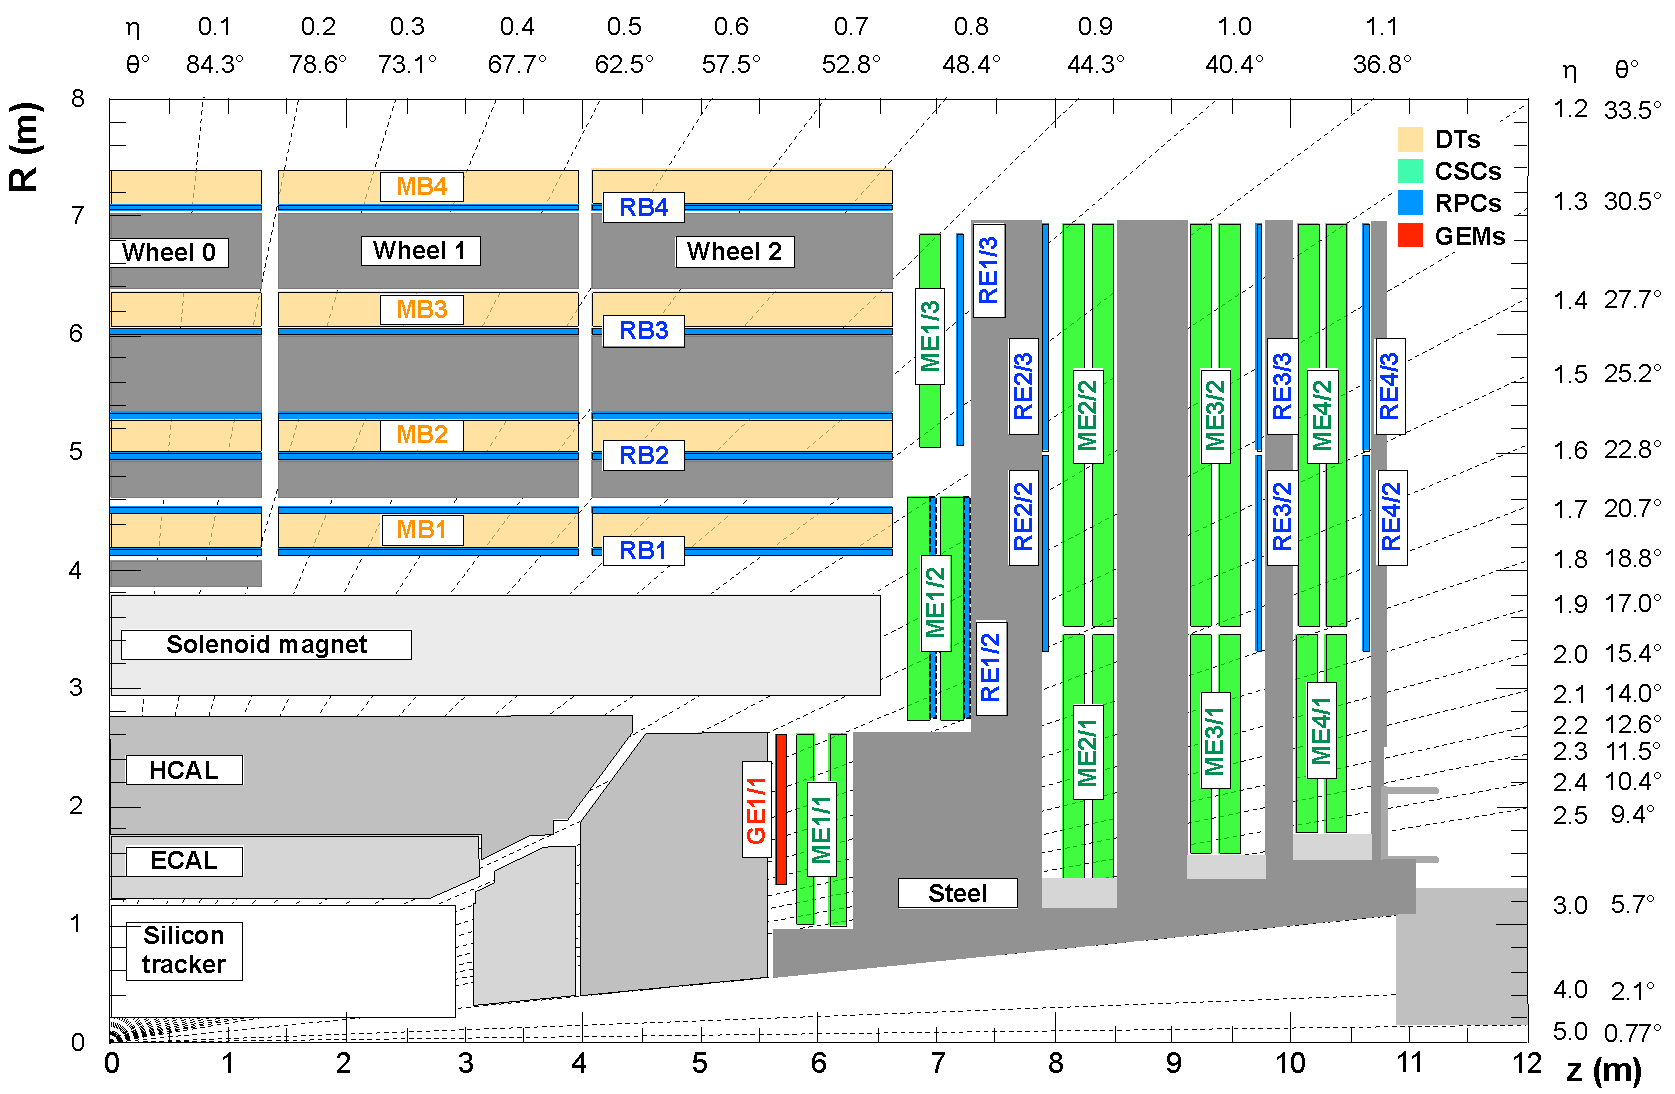
\includegraphics[width=\textwidth]{img/II-1-gem/ge11-quadrant.pdf}
      \caption{Schematic representation of a quadrant of CMS highlighting the location of the GE1/1 detector in red within the muon spectrometer \cite{Colaleo:2021453}.}
      \label{fig:II-1-gem-ge11}
    \end{figure}

  \section{Technology Overview}

  \section{Technical Design of GE1/1 chambers for CMS}

  \section{GE1/1 Prototyping Results}

  \section{Detector Design Evolution}

  \section{GEM Upgrade Schedule}
